\documentclass[12pt,a4paper]{article}
\usepackage[utf8]{inputenc}
\usepackage[T2A]{fontenc}
\usepackage[russian, english]{babel}
\usepackage{graphicx}
\usepackage{listings}
\begin{document}
\section{Постановка задачи}
Цели лабораторной работы:
\begin{enumerate}
    \item Получить физическую модель базы данных для выбранной предметной области.
    \item Сформулировать возможные запросы к базе даных.
\end{enumerate}
\section{Построение физической модели базы данных}
\subsection{Физическая модель основных сущностей}
Для построения физической модели базы данных возьмем за основу уже построенную в Lab1 логическую модель базы данных. \par
\begin{figure}[ht]
    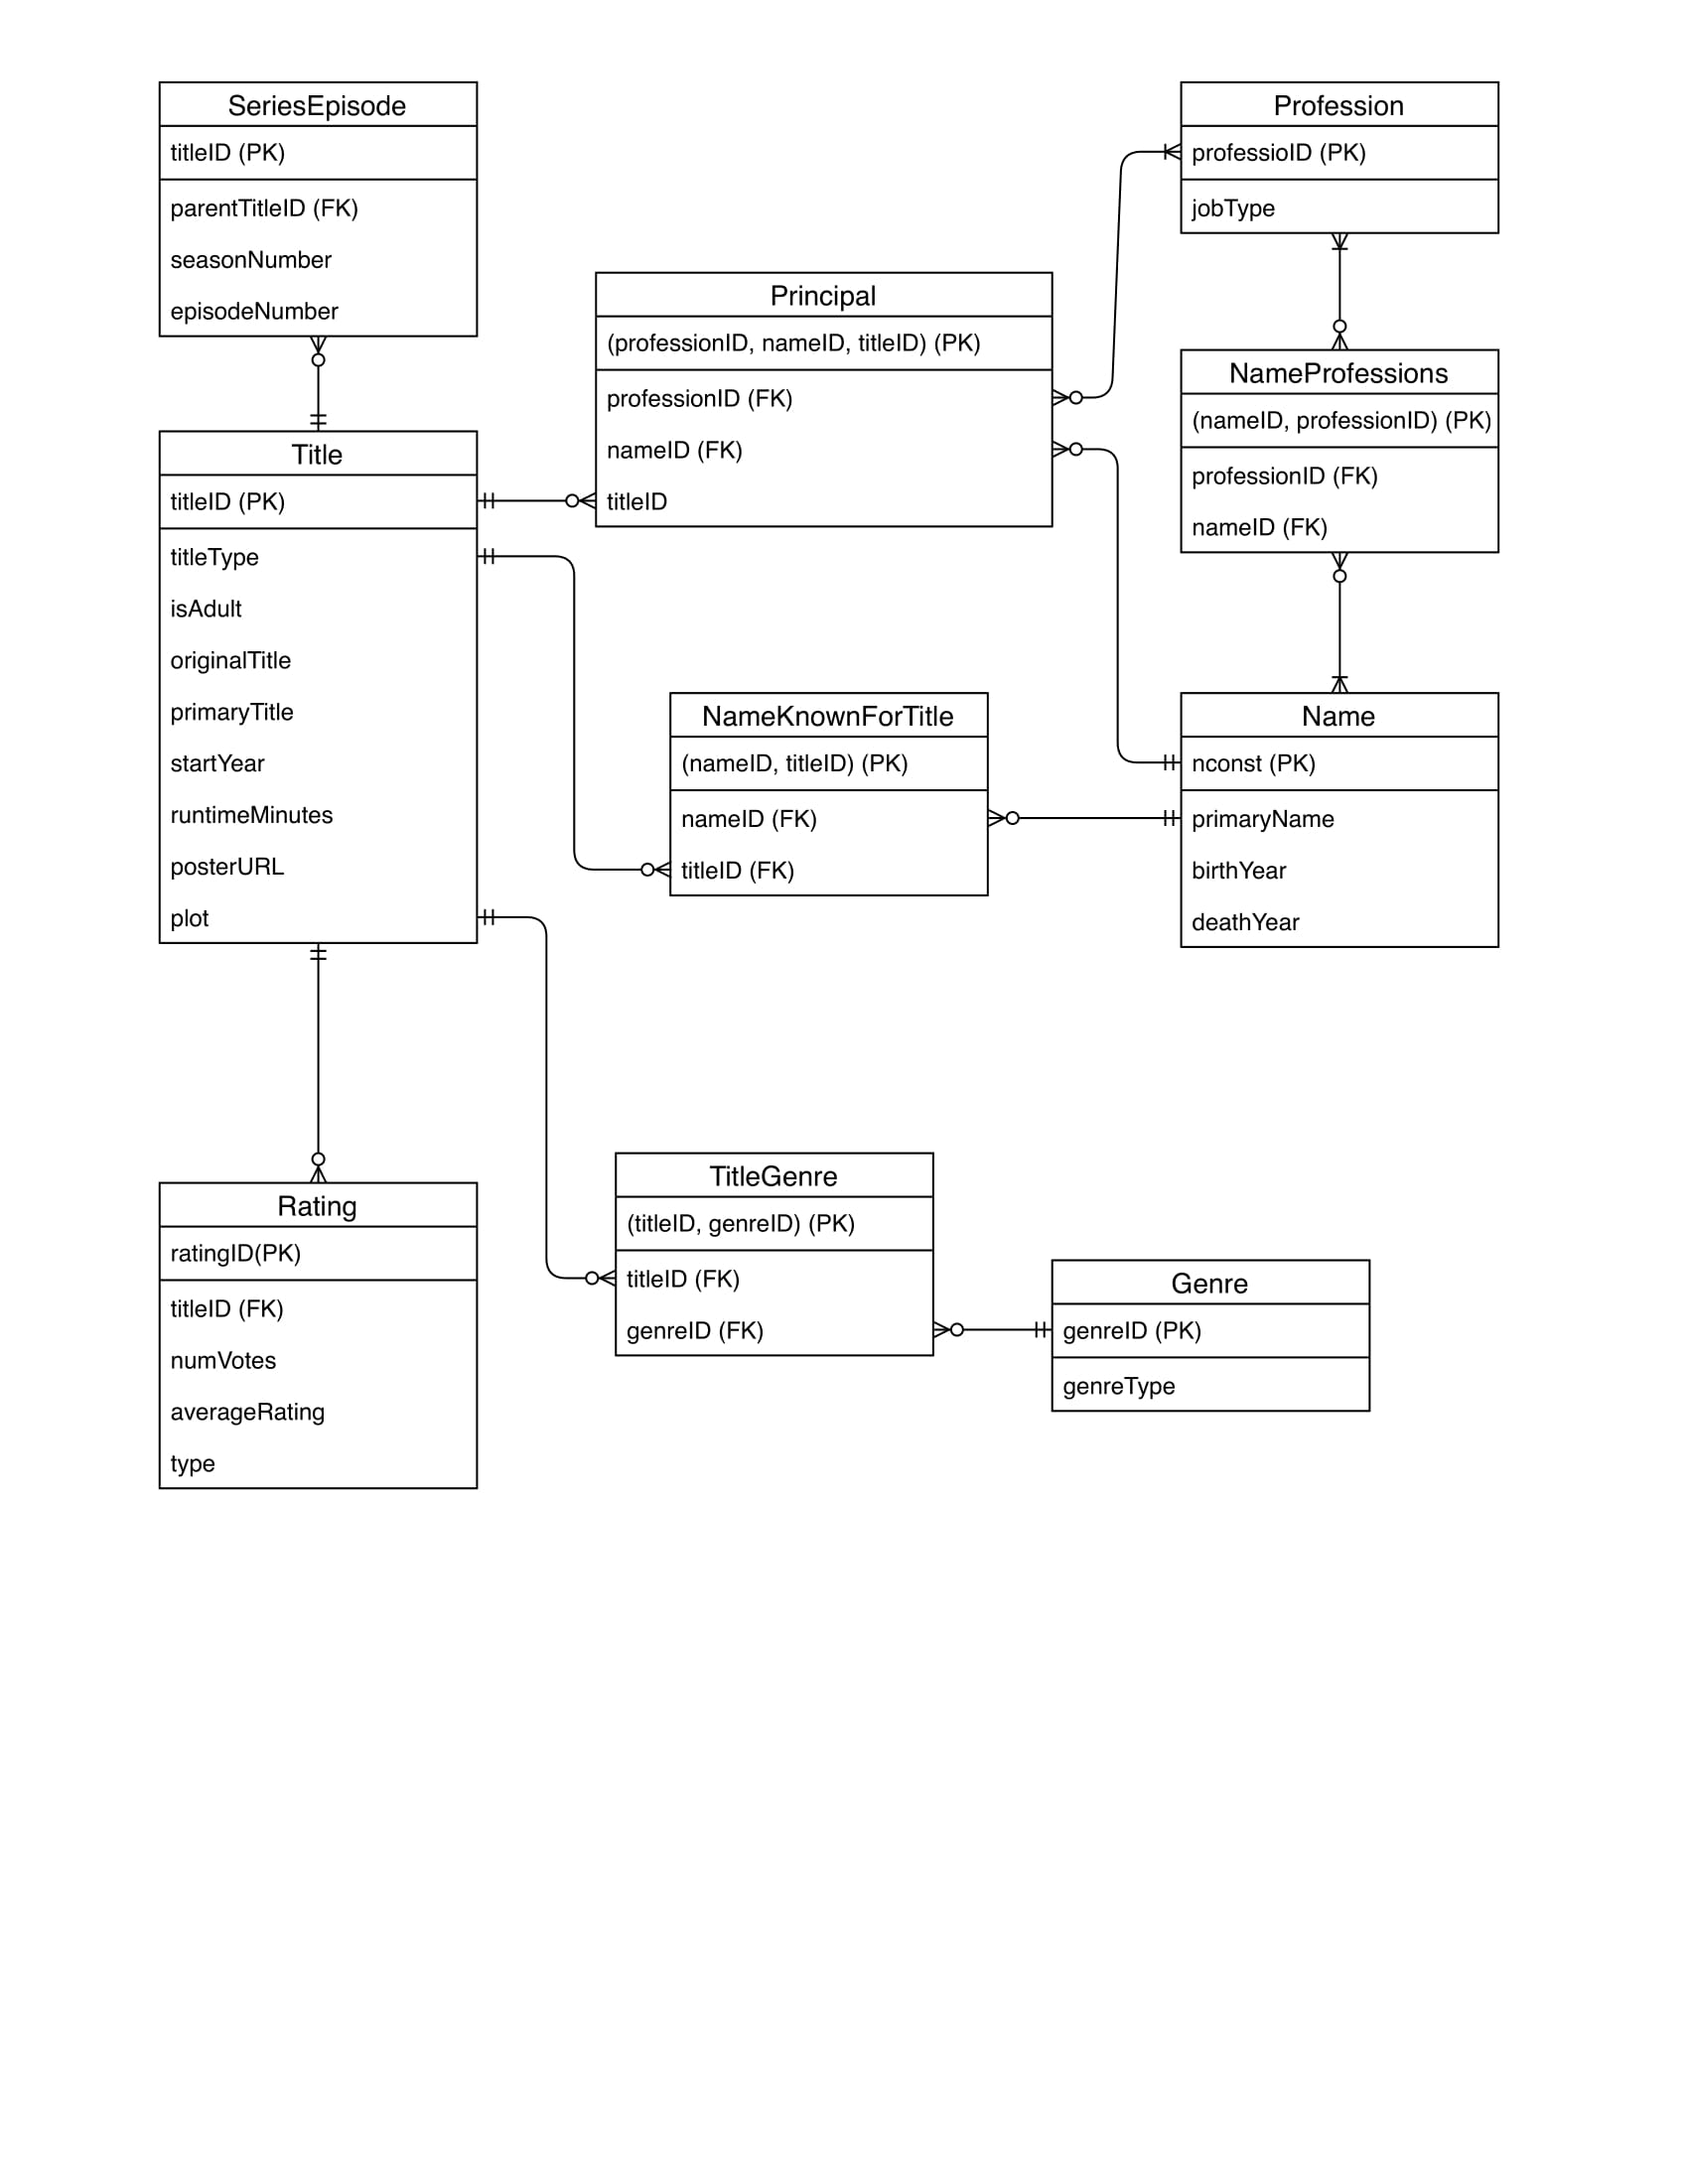
\includegraphics[width=\linewidth]{images/Lab1/logical_model.jpg}
    \caption{Logical model}
    \label{fig:Logical model}
\end{figure}
Определимся с типами атрибутов для сущности произведение киноиндустрии(Title):
\begin{enumerate}
    \item \textbf{titleID} - CHAR(9).
    \item \textbf{titleType} – ENUM(movie, tvSeries, etc.)
    \item \textbf{primaryTitle} – VARCHAR.
    \item \textbf{originalTitle} - VARCHAR.
    \item \textbf{isAdult} - BOOLEAN (BIT(1)).
    \item \textbf{startYear} – YEAR.
    \item \textbf{runtimeMinutes} – TINYINT UNSIGNED NOT NULL.
    \item \textbf{posterURL} - VARCHAR NULLABLE.
    \item \textbf{plot} - TEXT NULLABLE.
\end{enumerate} \par
\begin{lstlisting}[language=SQL]
CREATE TABLE `imdb_db`.`title` (
  `title_ID` CHAR(9) NOT NULL,
  `title_type` TEXT NOT NULL,
  `primary_title` TEXT NOT NULL,
  `original_title` TEXT NOT NULL,
  `isAdult` BIT(1) NOT NULL,
  `startYear` YEAR NOT NULL,
  `runtimeMinutes` SMALLINT UNSIGNED NOT NULL,
  `posterURL` TEXT NULL,
  `plot` TEXT NULL,
  PRIMARY KEY (`title_ID`));
\end{lstlisting}
Определимся с типами атрибутов для сущности рейтинг(Rating):
\begin{enumerate}
    \item \textbf{ratingID} - PK(titleID, ratingType).
    \item \textbf{titleID} - CHAR(9) NOT NULL.
    \item \textbf{averageRating} - DOUBLE UNSIGNED NOT NULL.
    \item \textbf{numVotes} - INT UNSIGNED NOT NULL.
    \item \textbf{ratingType} - ENUM(IMDB, Metacritic, etc.) NOT NULL.
\end{enumerate} \par
\begin{lstlisting}[language=SQL]
CREATE TABLE `imdb_db`.`rating` (
  `titleID` CHAR(9) NOT NULL,
  `numVotes` INT UNSIGNED NOT NULL DEFAULT 0,
  `averageRating` DOUBLE UNSIGNED NOT NULL DEFAULT 0,
  `ratingType` ENUM('IMDB', 'METACRITIC') NOT NULL,
  PRIMARY KEY (`titleID`, `ratingType`),
  CONSTRAINT `rating_titleID_FK` 
    FOREIGN KEY (`titleID`)
    REFERENCES `imdb_db`.`title`(`titleID`) 
    ON DELETE CASCADE
    ON UPDATE NO ACTION);
\end{lstlisting}
Определимся с типами атрибутов для сущности жанр(GENRE):
\begin{enumerate}
    \item \textbf{genreID} - TINYINT AUTOINCREMENT UNSIGNED.
    \item \textbf{genreType} - ENUM(Drama, comedy, etc.).
\end{enumerate} \par
\begin{lstlisting}[language=SQL]
CREATE TABLE `imdb_db`.`genre` (
  `genreID` TINYINT UNSIGNED NOT NULL AUTO_INCREMENT,
  `genre` ENUM('Action', 'Comedy', etc.) NOT NULL,
  PRIMARY KEY (`genreID`),
  UNIQUE INDEX `idgenre_UNIQUE` (`genreID` ASC));
\end{lstlisting}
Определимся с типами атрибутов для сущности эпизод сериала(SeriesEpisode):
\begin{enumerate}
    \item \textbf{titleID} - CHAR(9).
    \item \textbf{parentTitleID} - CHAR(9)
    \item \textbf{seasonNumber} - TINYINT UNSIGNED.
    \item \textbf{episodeNumber} - TINYINT UNSIGNED.
\end{enumerate} \par
\begin{lstlisting}[language=SQL]
CREATE TABLE `imdb_db`.`series_episode` (
  `titleID` CHAR(9) NOT NULL,
  `parentTitleID` CHAR(9) NOT NULL,
  `seasonNumber` TINYINT UNSIGNED NOT NULL,
  `episodeNumber` TINYINT UNSIGNED NOT NULL,
  PRIMARY KEY (`titleID`),
  CONSTRAINT `series_episode_titleID_FK` 
    FOREIGN KEY (`parentTitleID`)
    REFERENCES `imdb_db`.`title`(`titleID`) 
    ON DELETE CASCADE
    ON UPDATE NO ACTION);
\end{lstlisting}
Определимся с типами атрибутов для сущности деятель киноиндустрии(Name):
\begin{enumerate}
    \item \textbf{nameID} - VARCHAR(10).
    \item \textbf{primaryName} - TEXT.
    \item \textbf{birthYear} - DATE.
    \item \textbf{deathYear} - DATE.
\end{enumerate} \par
\begin{lstlisting}[language=SQL]
CREATE TABLE `imdb_db`.`name` (
  `nameID` CHAR(10) NOT NULL,
  `primaryName` TEXT NOT NULL,
  `birthDate` DATE NOT NULL,
  `deathDate` DATE NULL,
  PRIMARY KEY (`nameID`));
\end{lstlisting}
Определимся с типами атрибутов для сущности профессия(Profession):
\begin{enumerate}
    \item \textbf{professionID} - TINYINT AUTOINCREMENT UNSIGNED.
    \item \textbf{jobType} - ENUM(director, writer, etc.).
\end{enumerate} \par
\begin{lstlisting}[language=SQL]
CREATE TABLE `imdb_db`.`profession` (
  `professionID` TINYINT NOT NULL AUTO_INCREMENT,
  `profession` ENUM('Director', 'Writer', etc.) NOT NULL,
  PRIMARY KEY (`professionID`));
\end{lstlisting}
\subsection{Реализация связывающих таблиц}
Создадим промежуточную таблицу titleGenre для реализации связи 
многие ко многим между сущностями Title и Genre.

\begin{lstlisting}[language=SQL]
CREATE TABLE `imdb_db`.`title_genre` (
  `titleID` CHAR(9) NOT NULL,
  `genreID` TINYINT UNSIGNED NOT NULL,
  PRIMARY KEY (`titleID`, `genreID`),
  CONSTRAINT `title_genre_titleID_FK`
    FOREIGN KEY (`titleID`) 
    REFERENCES `imdb_db`.`title`(`titleID`) 
    ON DELETE CASCADE 
    ON UPDATE NO ACTION,
  CONSTRAINT `title_genre_genreID_FK` 
    FOREIGN KEY (`genreID`)
    REFERENCES `imdb_db`.`genre`(`genreID`) 
    ON DELETE CASCADE 
    ON UPDATE NO ACTION);
\end{lstlisting}

Создадим промежуточную таблицу nameKnownForTitle для реализации связи 
многие ко многим между сущностями Name и Title.

\begin{lstlisting}[language=SQL]
CREATE TABLE `imdb_db`.`name_known_for_title` (
  `nameID` CHAR(10) NOT NULL,
  `titleID` CHAR(9) NOT NULL,
  PRIMARY KEY (`nameID`, `titleID`),
  CONSTRAINT `name_known_for_title_nameID_FK` 
  FOREIGN KEY (`nameID`)
    REFERENCES `imdb_db`.`name`(`nameID`)
    ON DELETE CASCADE
    ON UPDATE NO ACTION,
  CONSTRAINT `name_known_for_title_titleID_FK` 
  FOREIGN KEY (`titleID`)
    REFERENCES `imdb_db`.`title`(`titleID`)
    ON DELETE CASCADE
    ON UPDATE NO ACTION);
\end{lstlisting}

Создадим промежуточную таблицу nameProfessions для реализации связи 
многие ко многим между сущностями Name и Profession.

\begin{lstlisting}[language=SQL]
CREATE TABLE `imdb_db`.`name_professions` (
  `nameID` CHAR(10) NOT NULL,
  `professionID` TINYINT NOT NULL,
  PRIMARY KEY (`nameID`, `professionID`),
  CONSTRAINT `name_professions_nameID_FK` 
  FOREIGN KEY (`nameID`)
    REFERENCES `imdb_db`.`name`(`nameID`)
    ON DELETE CASCADE
    ON UPDATE NO ACTION,
  CONSTRAINT `name_professions_professionID_FK` 
  FOREIGN KEY (`professionID`)
    REFERENCES `imdb_db`.`profession`(`professionID`)
    ON DELETE CASCADE
    ON UPDATE NO ACTION);
\end{lstlisting}

Создадим промежуточную таблицу principal для реализации связи 
многие ко многим между сущностями Name, Profession и Title.

\begin{lstlisting}[language=SQL]
CREATE TABLE `imdb_db`.`principal` (
  `titleID` CHAR(9) NOT NULL,
  `nameID` CHAR(10) NOT NULL,
  `professionID` TINYINT NOT NULL,
  PRIMARY KEY (`titleID`, `nameID`, `professionID`),
  CONSTRAINT `principal_titleID_FK` 
  FOREIGN KEY (`titleID`)
    REFERENCES `imdb_db`.`title`(`titleID`)
    ON DELETE CASCADE
    ON UPDATE NO ACTION,
  CONSTRAINT `principal_nameID_FK` 
  FOREIGN KEY (`nameID`)
    REFERENCES `imdb_db`.`name`(`nameID`)
    ON DELETE CASCADE
    ON UPDATE NO ACTION,
  CONSTRAINT `principal_professionID_FK` 
  FOREIGN KEY (`professionID`)
    REFERENCES `imdb_db`.`profession`(`professionID`)
    ON DELETE CASCADE
    ON UPDATE NO ACTION);      
\end{lstlisting}
\begin{figure}[ht]
  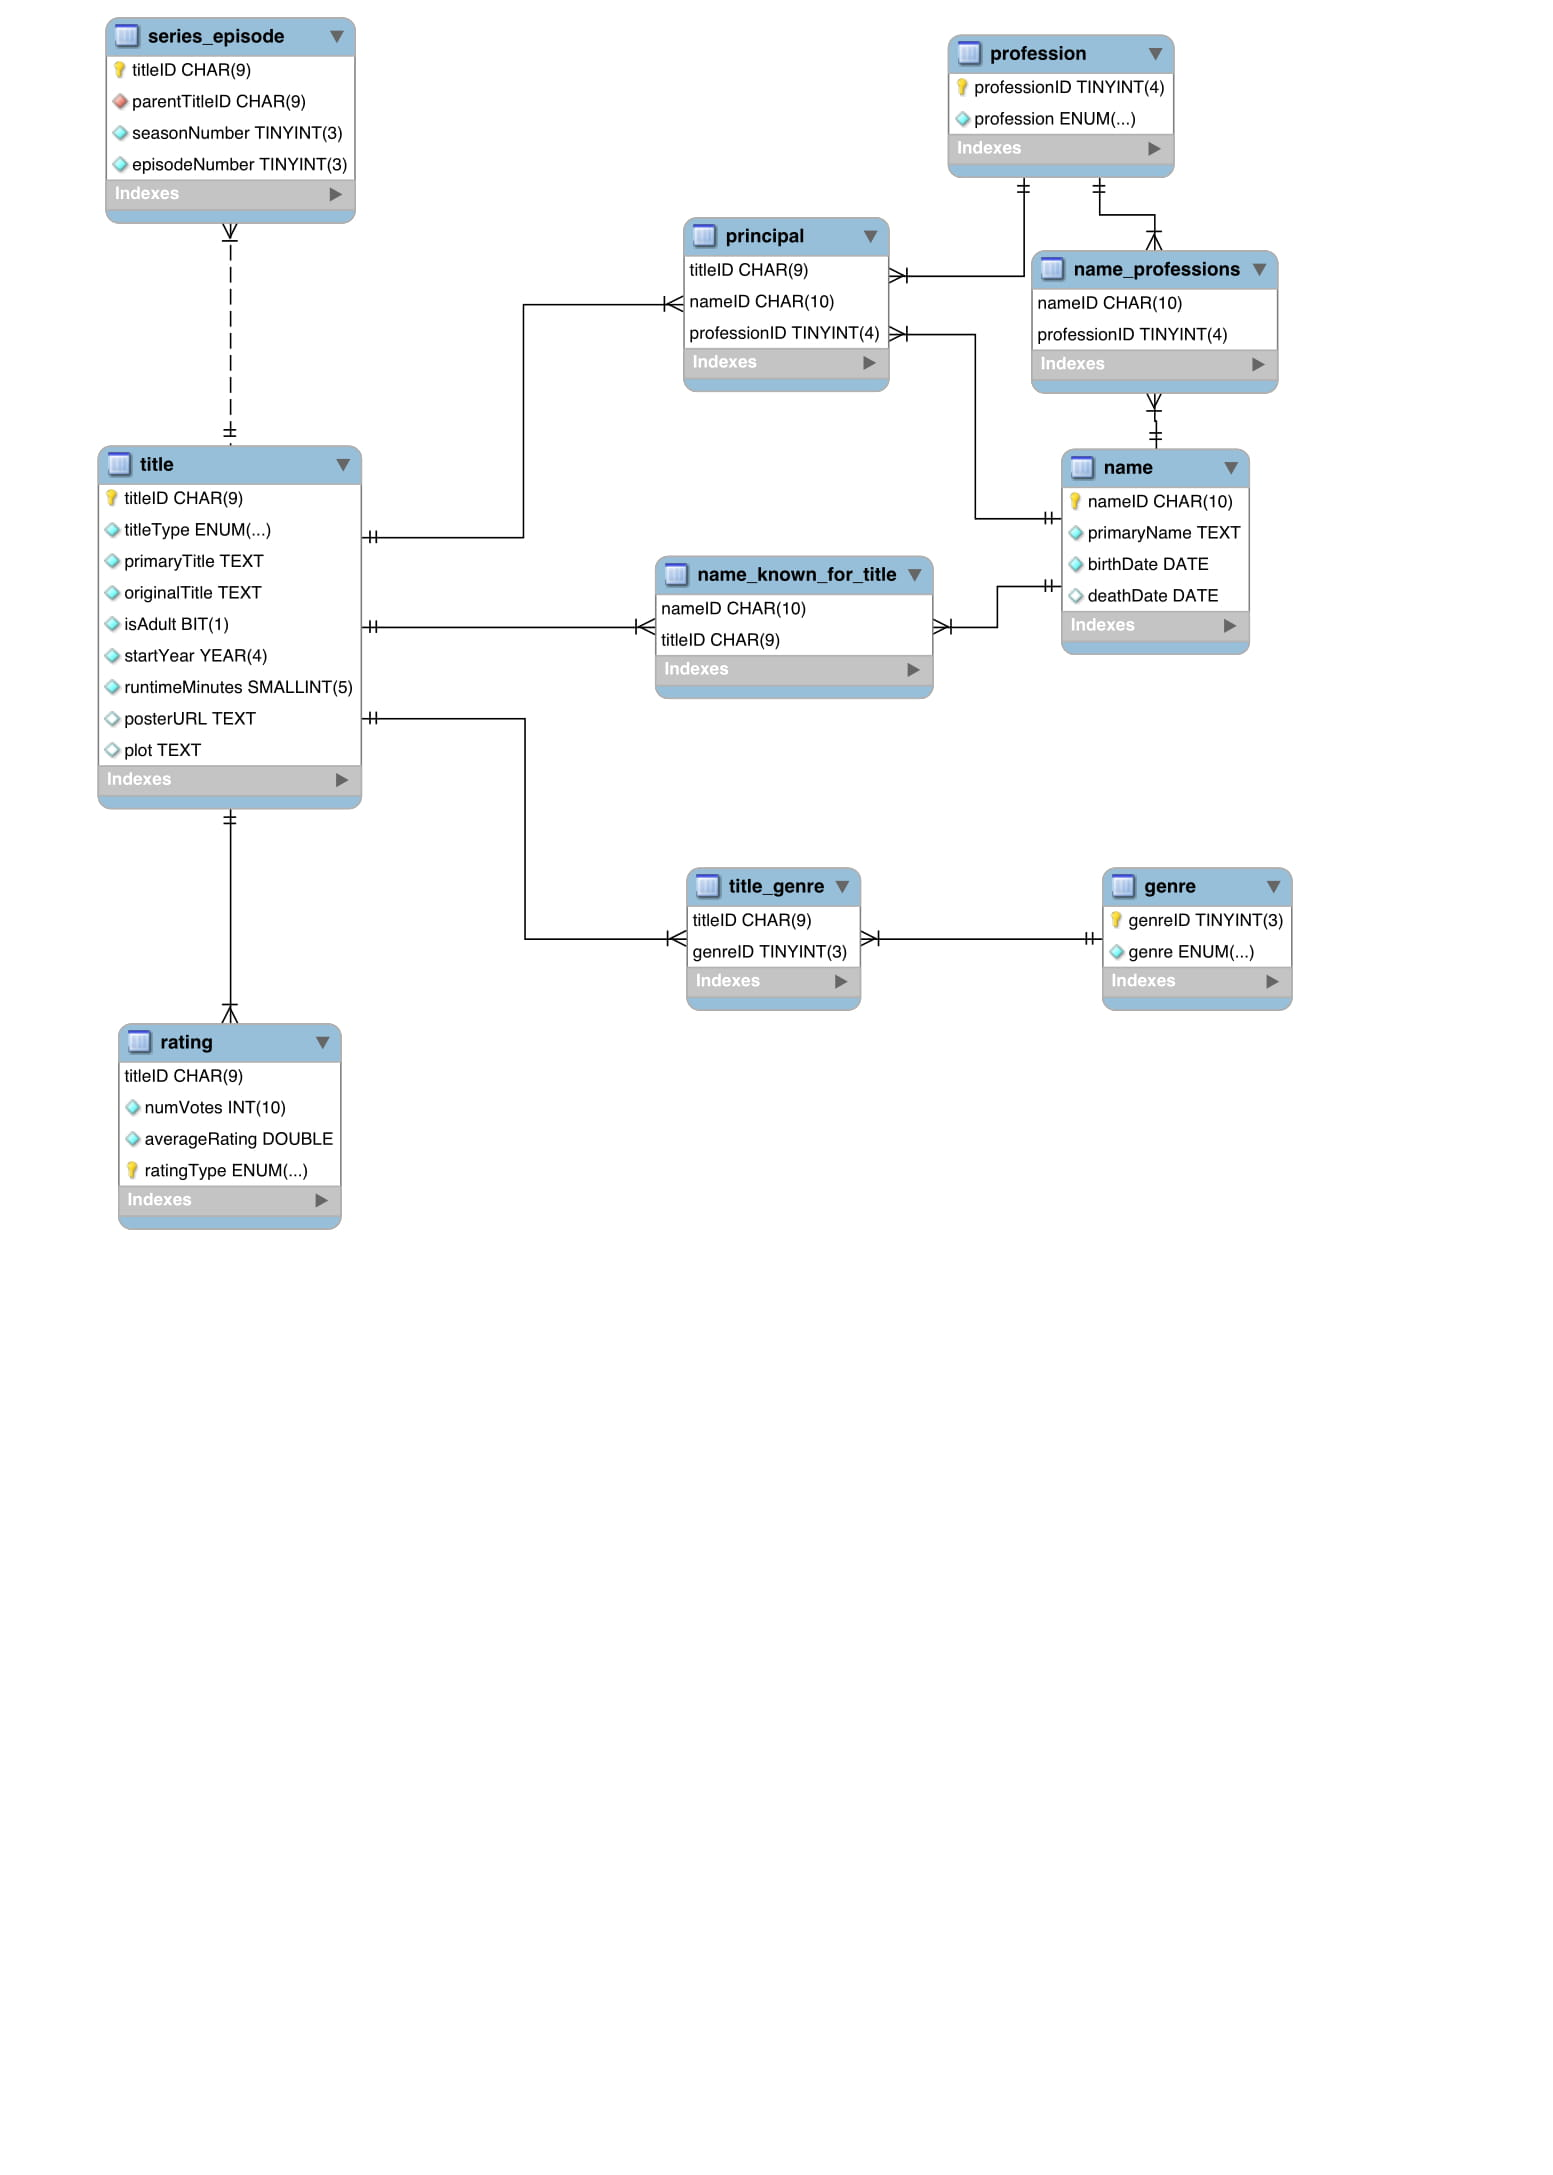
\includegraphics[width=\linewidth]{images/Lab2/physical_model.jpg}
  \caption{Physical model}
  \label{fig:Physical model}
\end{figure}
\section{Используемые источники}
\begin{enumerate}
    \item https://dev.mysql.com/doc/refman/8.0/en/charset.html
    \item https://dev.mysql.com/doc/refman/8.0/en/data-types.html
    \item https://www.mysqldatatypes.com/
    \item https://dev.mysql.com/doc/refman/8.0/en/create-table.html
    \item https://dev.mysql.com/doc/refman/8.0/en/create-table-foreign-keys.html
\end{enumerate}
\end{document}